
%(BEGIN_QUESTION)
% Copyright 2006, Tony R. Kuphaldt, released under the Creative Commons Attribution License (v 1.0)
% This means you may do almost anything with this work of mine, so long as you give me proper credit

An alternative to using a pressure-relief valve to control pressure in a hydraulic system is to use a {\it variable-displacement pump} with hydraulic feedback:

$$\includegraphics[width=15.5cm]{i00763x01.eps}$$

As hydraulic pressure increases, the pump mechanism automatically adjusts to give less volume displacement per rotation.  Explain how this works to regulate pressure, and also why it saves energy compared to the more traditional design of a constant-displacement pump combined with a pressure-relief valve.

\underbar{file i00763}
%(END_QUESTION)





%(BEGIN_ANSWER)

Instead of wasting unused hydraulic energy in a pressure relief valve, this system reduces the amount of hydraulic energy input to the system when it is not needed.

\vskip 10pt

Follow-up question: a common design of variable-displacement hydraulic pump (and motor!) is the {\it swash plate} style, where the angle of the swash plate changes to alter the pump's per-revolution displacement.  Research this pump design and explain how it works.

%(END_ANSWER)





%(BEGIN_NOTES)

%INDEX% Mechanics, fluid power systems: variable displacement pump for pressure regulation

%(END_NOTES)


